
\subsection{Further optimizing code yields large single-threaded speedups}

\osprey3's code has been heavily optimized to improve single-threaded performance. Two main areas have received the most attention, and the most improvement in performance, so far: A* search speed, and conformation minimization speed.

The performance of A* search in \osprey depends mostly on the size of the conformation space of the design. More mutable and flexibile residues create a larger conformation space which must be searched systematically to find the lowest-energy conformations while perserving guarantees on solution quality, and hence the search requires more time. Search time is also dependent on the speed at which we can execute the scoring functions on A* nodes. Optimizations in \osprey3 have dramatically increased the A* node scoring speed mainly through the re-use of computed values between different nodes. Many intermediate values used by the A* scoring functions need only be computed once per design and can be cached throughout the rest of the search. This reduces the cost of node scoring by roughly an order of magnitude. We can also score child nodes differentially against their parent nodes to speed up node scoring. Caching intermediate values during the parent node scoring and using them to simplify child node scoring yields roughly another order of magnitude speedup in A* node scoring. \jeff{trying to be concise here, hopefully we don't need the mathematical details of these A* scoring functions?}

\osprey3 also includes optimizations to improve the performance of forcefield evaluation and conformation minimization. The code in \osprey3 which evaluates forcefield energies for a protein conformation has been heavily optimized, although speed gains here over \osprey2 are modest (roughly two-fold), since the original code was already well-optimized in this area. Much larger performance increases were gained by caching forcefield parameters and lists of atom pairs between different conformations to be minimized yielded roughly a 10-fold increase in speed. \jeff{I'm going off of memory for the impact of these optimizations. Hopefully rough estimates are good enough here? Or maybe this is too much detail altogether?}

Combined together, these optimizations to single-threaded performance made \osprey3 about 425-fold faster than \osprey2 on a small benchmark sidechain packing problem (See Figure~\ref{fig:speedup}).

\begin{figure}\label{fig:speedup}
\center
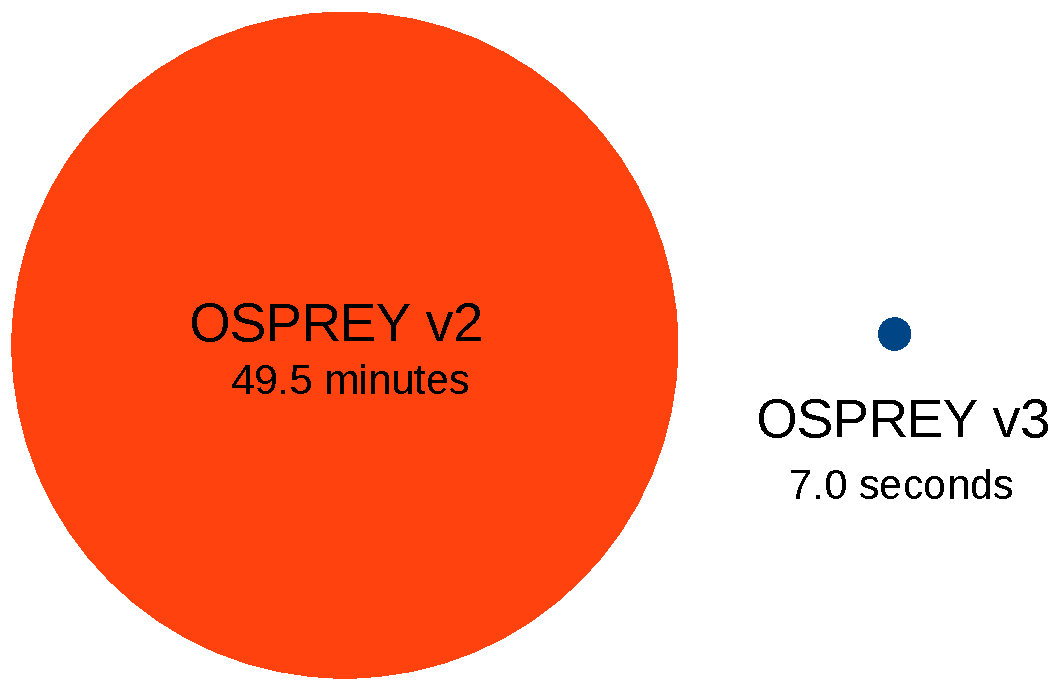
\includegraphics[width=2in]{figures/speedup.pdf}
\caption{On a small benchmark sidechain packing problem involving a 114-residue fragment of PDZ3 domain of PSD-95 protein complexed with a 6-residue peptide ligand (PDB ID: 1TP5) and consisting of six continuously flexible residues, \osprey3 (blue) finished the design 425-fold faster than \osprey2 (red). Runtimes for the benchmark design are represented as the areas of the discs. A smaller disc represents a faster runtime. This benchmark was performed in a single thread running on an Intel Xeon E5-2640 v4 CPU.}
\end{figure}
